\documentclass[UTF8,a4paper,12pt]{ctexart}%需要UTF8编码

\bibliographystyle{gbt7714-2005} %参考文献格式设为GBT7714-2005N.bst
\newcommand{\upcite}[1]{\textsuperscript{\textsuperscript{\cite{#1}}}}
\usepackage{url}

\usepackage[draft=false,colorlinks=true,CJKbookmarks=true,linkcolor=black,citecolor=green,urlcolor=blue]{hyperref} %参考文献跳转,此宏包会自动载入graphicx

\usepackage[top=3cm,bottom=2cm,left=2cm,right=2cm]{geometry} % 页边距

\usepackage{longtable}%生成跨页的表格
\usepackage{array} % for extrarowheight
\setlength{\extrarowheight}{1.5pt}


\usepackage[american]{babel}%它的引用是遇单词换行的时候,确保单词的切割是按照音节来而不是随意切割。这会让作为native speaker的审稿人赏心悦目,心中暗爽。
\usepackage{microtype}%它的最大特点就是能够调整全篇文章(或局部)的字间距,字间距最大调整范围为±1em。可使得某段落不会出现单独一个单词占一行,或文章末尾单独一行文字占一页的不美观情况(注,该包在NIPS中自带引用;而ECCV由于LNCS在排版方面的一些限制因素,不推荐在ECCV中使用该包引用);
\addto\captionsamerican{
	\renewcommand\contentsname{目录} 
	\renewcommand\listfigurename{插图目录} 
	\renewcommand\listtablename{表格目录} 
	\renewcommand\refname{参考文献} 
	\renewcommand\indexname{索引} 
	\renewcommand\figurename{图} 
	\renewcommand\tablename{表} 
	\renewcommand\abstractname{摘要} 
	\renewcommand\partname{部分} 
	\renewcommand\appendixname{附录} 
	\renewcommand\today{\number\year年\number\month月\number\day日} 
}

%\setCJKmainfont{STKaitiSC-Regular} %中文字体

\usepackage{pdfpages}%插入封面

\usepackage{latexsym}

\usepackage{fancyhdr}
\pagestyle{fancy}
\lhead{\bfseries \leftmark}
\chead{}
\rhead{\thepage}
%\cfoot{姓名 16300000001}
\lfoot{}
\rfoot{}
\renewcommand{\headrulewidth}{0.4pt}
%\renewcommand{\footrulewidth}{0.4pt}
\title{相控阵雷达角度测量}
\author{韩宙 22112020088}
\date{}

\usepackage{listings}
\usepackage{color}
\definecolor{dkgreen}{rgb}{0,0.6,0}
\definecolor{gray}{rgb}{0.5,0.5,0.5}
\definecolor{mauve}{rgb}{0.58,0,0.82}
\lstset{ %
  language=Octave,                % the language of the code
  basicstyle=\footnotesize,           % the size of the fonts that are used for the code
  numbers=left,                   % where to put the line-numbers
  numberstyle=\tiny\color{gray},  % the style that is used for the line-numbers
  stepnumber=1,                   % the step between two line-numbers. If it's 1, each 
  %line 
                                  % will be numbered
  numbersep=5pt,                  % how far the line-numbers are from the code
  backgroundcolor=\color{white},      % choose the background color. You must 
  %add \usepackage{color}
  showspaces=false,               % show spaces adding particular underscores
  showstringspaces=false,         % underline spaces within strings
  showtabs=false,                 % show tabs within strings adding particular 
  %underscores
  frame=single,                   % adds a frame around the code
  rulecolor=\color{black},        % if not set, the frame-color may be changed on 
  %line-breaks within not-black text (e.g. commens (green here))
  tabsize=2,                      % sets default tabsize to 2 spaces
  captionpos=b,                   % sets the caption-position to bottom
  breaklines=true,                % sets automatic line breaking
  breakatwhitespace=false,        % sets if automatic breaks should only happen at 
  %whitespace
  title=\lstname,                   % show the filename of files included with 
  %\lstinputlisting;
                                  % also try caption instead of title
  keywordstyle=\color{blue},          % keyword style
  commentstyle=\color{dkgreen},       % comment style
  stringstyle=\color{mauve},         % string literal style
  escapeinside={\%*}{*)},            % if you want to add LaTeX within your code
  morekeywords={*,...}               % if you want to add more keywords to the set
}
  
\begin{document}
	 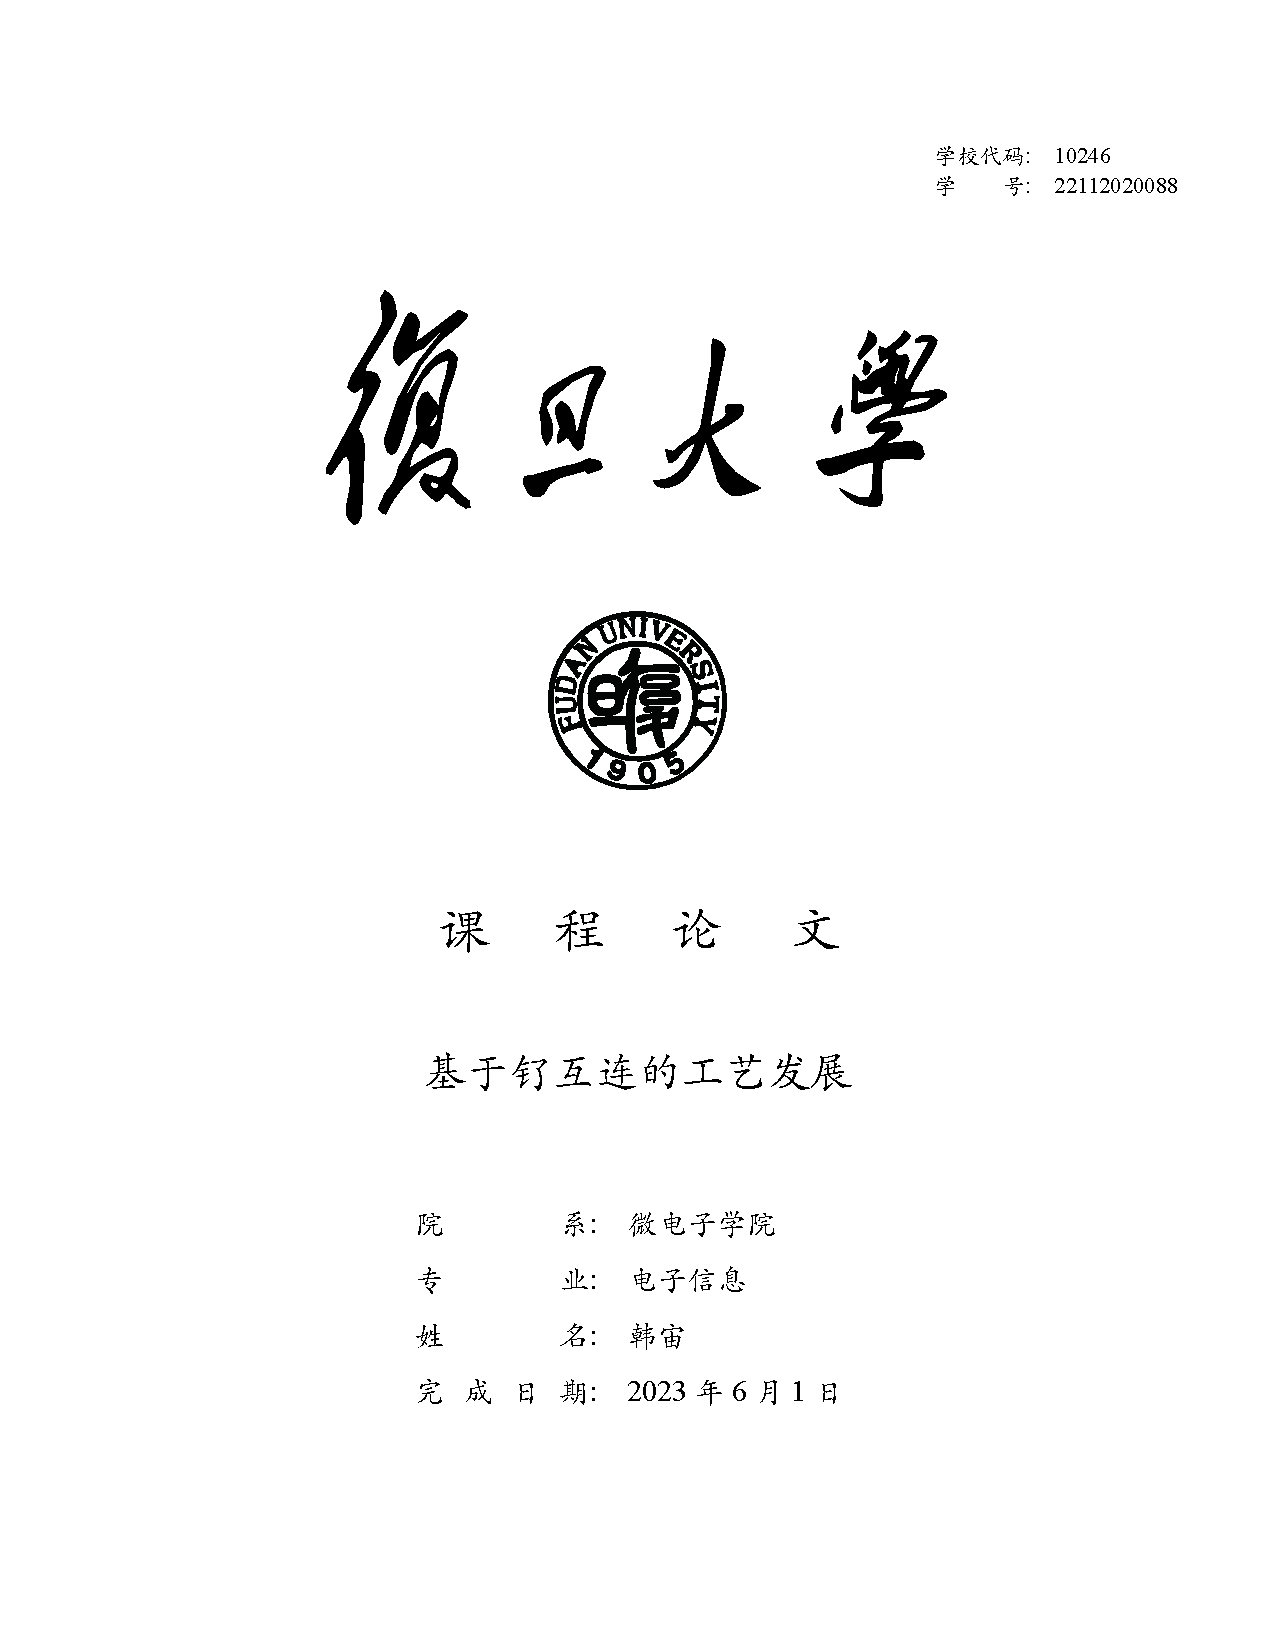
\includepdf{Book-Cover.pdf}   %// 是否带封面
%\maketitle
\newpage
\begin{abstract}
	互联工艺中Al逐渐被Cu取代,因为铜的电阻率更小,抗电迁移性能更强,但是Cu互连的问题
	也很突出,就是在高温退火的条件下,很容易向Si中扩散形成铜的硅化物,极大的提升电阻率。为了
	克服Cu互连扩散的问题,一般采用预先生长一层Ta/TaN作为铜扩散的阻挡层和粘附层,来防止
	Cu在高温退火条件下扩散。


	随着集成电路特征尺寸的不断缩小,集成电路先进技术介电已经发展到10nm及以下,
	传统的Ta/TaN体系已经不能满足工艺发展的需要。
	。Ru、Co、Mo等一些新型合金材料由于具备较低的电阻率、与Cu的粘附性好等优点,
	被用来研究作为下一代的粘附层或者阻挡层材料。这些材料相对于Ta的优势是电导率相对较高
	可以不需要PVD生长籽晶层,直接进行Cu互连中的Cu电镀。


	本文中主要介绍了Ru金属作为阻挡层材料的基本性质、优势与劣势,回顾Ru金属作为阻挡层材料的发展
	最后应用Ru金属的对于Cu的黏附性高而对于Si黏附性较差的以及电阻率低而具备的可以直接电镀铜的优势
	将Ru金属应用在新的工艺中,从而备受关注。
\end{abstract}
\noindent\zihao{4}\textbf{关键词}\quad\zihao{-4} Ru互连;阻挡层;Cu互连;ALD技术
\newpage
\tableofcontents %生成目录




\listoffigures% 插图目录
\setcounter{page}{0}
\thispagestyle{empty}
\newpage

\section{铜互连阻挡层简介}
\subsection{集成电路技术发展}
集成电路技术(IC)是实现当今社会数字化与智能化的技术基础,它促进了社会
的经济繁荣,提升了现代科技水平。当前,依托于信息技术及软件技术的快速发展,
集成电路技术也在其带领下得到了快速的更新,逐渐引领未来人工智能技术及计算机
网络技术的前行。表 1.1 展示了 IC 在每个发展阶段的集成度,自 20 世纪 60 年代
起,集成电路的集成度经历了从 1 个元件到至今超过 10
9个元件的发展历程,逐渐实现了全球大规模的发展,形成了全新的技术产业链,与此同时,芯片制造也正在向晶
圆代工进行转变。


迄今为止,IC 芯片的集成度已超过十亿,进入了极大规模集成电路(GLSI)发
展的时代,并且摩尔定律依然在 IC 中延续,每隔 18 个月芯片上元器件的数量就上升
一倍,这使得 IC 集成度不断提高,互连线层数不断增加,对集成电路晶圆加工精度
的要求也就越来越高。2018 年中美贸易争端,更凸显了集成电路芯片制造技术的
极端重要性。因此,为了拉近与国际顶尖水平的差距,并摆脱我国高端精密芯片依赖
进口的现状,开展 10 nm 及以下 IC 技术节点的研发对促进我国微电子技术发展具有
重大意义。


\subsection{Cu互连技术}
随着集成电路特征尺寸的持续缩小,铝(Al)布线所引起的互连电阻及 RC 延迟
不断增加,这限制了集成电路的发展。1997 年,IBM 公司利用双大马士革工艺完成
了 Cu 互连技术,Cu 互连技术是指在集成电路互连层的制造中,采用 Cu 金属取代传
统的 Al 金属作为布线材料。铜互连技术相对于铝互连有着诸多的优势,首先,Cu 具
有比 Al 更低的电阻率,这可以极大地缩短 RC 延迟时间;其次,铜互连技术采用碳掺
杂 SiO2材料取代传统的 SiO2成为互连线之间的隔离层,这极大地削减了互连层厚度,
降低了互连电容,并提高了器件的灵敏度;最后,IC 芯片在使用过程中由于布线材料
过热会出现电子迁移现象,严重影响了产品的质量,而 Cu 相对于 Al 具有更高的熔
点(Cu∼1083℃,Al∼660℃),有效降低了布线金属电子迁移的频率,提高了产品
的良率及可靠性。因此,Cu 互连技术及工艺在 IC 晶圆制造过程中的应用逐渐得到应用。


\subsection{Cu阻挡层技术}
Cu阻挡层是指使用铜(Cu)材料作为阻挡层的一种技术,用于集成电路制造中。铜具有
良好的电导性能,但在一些情况下,它可能会扩散到其他层,引起电路的故障。为了解决
这个问题,Cu阻挡层被引入到集成电路的制造过程中。


钨是最早用于Cu互连阻挡层的材料之一。它具有良好的热稳定性和电阻率,可以有效阻止铜的扩散。
然而,钨的主要缺点是它的成本较高,而且在某些情况下可能与铜发生反应,导致电阻增加。


钽(Ta)是一种常用的阻挡层材料,在集成电路制造中被广泛应用。它具有以下几个优势,
抑制铜扩散能力:钽具有出色的抑制铜扩散能力。它可以有效地阻止铜从互连层扩散到其他层,
从而减少电路中的故障和损失。这是使用钽作为Cu互连阻挡层的主要优势之一。
优异的热稳定性:钽具有良好的热稳定性,可以在高温下保持其性能和结构的稳定。
这对于集成电路的制造和工作过程至关重要,因为制造过程中涉及到高温处理步骤,
而电路在使用过程中也会受到高温环境的影响。
电阻率适中:钽的电阻率适中,既不过高也不过低。这使得钽作为阻挡层材料时能够提供良好的
电导性能,同时避免信号传输延迟的增加。
与铜的兼容性:钽与铜具有较好的兼容性,不会发生显著的反应或相互扩散。这意味着钽阻挡层
可以与铜互连层紧密结合,形成稳定和可靠的界面。
可靠性和可制备性:钽材料具有良好的可靠性和可制备性,制造商可以使用现有的工艺和设备来
实现钽阻挡层的制备。这使得钽成为一种经济有效且可行的选择。而钽氮化物(TaN)在热稳定性
方面相对较好,能够承受高温处理和工作环境。因此,在高温应用中,Ta/TaN可能比纯钽更适合作为
阻挡层材料。


然而,为了满足铜技术节点不断缩小的需求,传统材料和工艺面临挑战。由于铜的高电阻率,
在Ta/TaN上直接电化学沉积是不现实的。因此,需要通过物理气相沉积(PVD)或化学气相沉积
(CVD)预沉积铜种子层,但铜种子层的不均匀性对现代20nm以下甚至10nm以下Cu技术节点的
无缺陷填充具有破坏性的影响。为了在纳米尺度上成功地超填充沟槽,需要具有超薄尺寸、高
电阻率和稳定性的新型铜扩散势垒材料。所以人们着力于开发新一代的Cu互连材料,其中Co,
Mo和Ru等金属备受关注,因为其在满足Cu阻挡层的性质外还由于其具有较低的电阻率可以直接
在阻挡层表面进行电镀。


新一代的阻挡层材料需要具备以下的理想条件包括:
\begin{enumerate}
	\item 对铜金属和介电层的粘附性
	\item 与铜的不混溶和防止铜在高温下的扩散能力
	\item 铜的直接接触具有良好的导电性
	\item 可以在介电层上的均匀沉积超薄膜
\end{enumerate}



只有满足这些条件才有可能被采用到新型的阻挡层材料之中,这里我们着重介绍Ru金属在Cu互连中的
发展与应用。

\section{Ru阻挡层}
Ru是一种空气稳定的金属,电阻率($\rho Ru =7.1\mu \Omega \cdot cm$)比Ta=
($\rho Ta =7.1\mu \Omega \cdot cm$)低得多,允许直接
电化学镀铜。更重要的是,Ru的熔点高达2334◦C,溶解度可以忽略不计,但与铜的润湿性极好,在高
温下对电镀铜具有良好的粘附性。因此,Ru被认为是替代传统扩散势垒材料的一种很有前途的候选材料。
Ru还可以通过PVD、CVD、ALD等气相沉积方法,可以将Ru阻挡层的薄膜放置在固体衬底上,湿法方式
生长例如电镀等。

如图\ref{Fig:1}所示,在Cu/Ru/Si体系中,经过恰当温度的退火Ru的电阻率最低可以达到
$3\mu \Omega \cdot cm$,同时体系的失效温度要超过$500^oC$,这就说明Ru作为阻挡层的潜力与稳定
性。


如图\ref{Fig:2}所示,由于Ru的电阻率极低,所以不需要任何的籽晶层Cu就可以直接在Ru表面进行
电镀同时需要的电压非常的低,在前几个循环的电镀中,其开路的电镀电压为0.5,而经过前几层铜电镀后
其需要的开路电压接近于0且在100层以上循环电镀生长过程中没有任何的变化,这就说明了Ru对于Cu直接
电镀的性能优越性与低损耗性。在实验中可以通过磁控溅射技术,可以在硅片上沉积的20nmRu薄膜上
并在Running表面电镀Cu层,其Cu ED效率高达95\%。



\begin{figure}[htb]
	\centering
	\begin{minipage}[t]{0.5\textwidth}
	\centering
	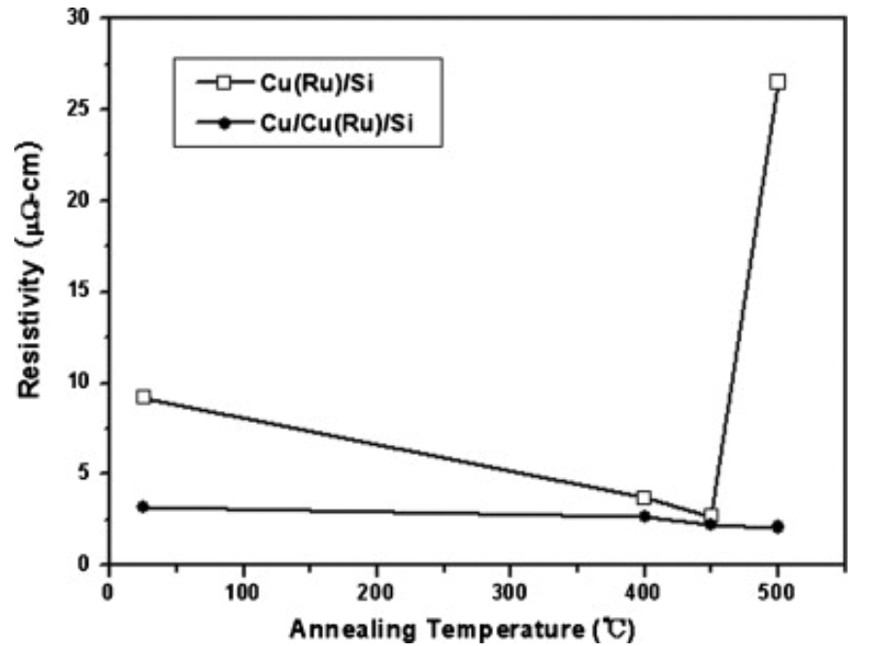
\includegraphics[width=0.8\textwidth]{1.jpg}
	\caption{Ru阻挡层在不同温度下退火的电阻率}
	\label{Fig:1}
	\end{minipage}
	\begin{minipage}[t]{0.45\textwidth}
	\centering
	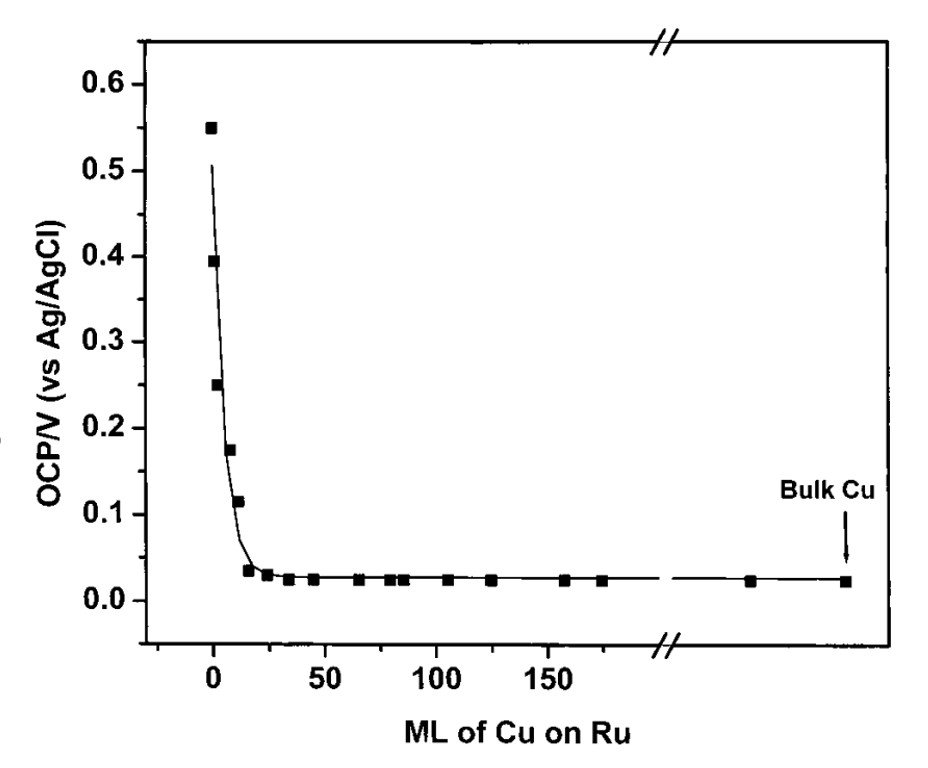
\includegraphics[width=0.8\textwidth]{2.jpg}
	\caption{Ru阻挡层直接电镀稳定性}
	\label{Fig:2}
	\end{minipage}
\end{figure}


\subsection{纯Ru阻挡层}

通过PVD溅射与铜电镀得到的$Cu/Ru/SiO_2$体系可以维持在高温退火的情况下不产生新的相且不互相扩散。
如图\ref{Fig:3}所示在室温情况下与在$600^oC$温度退火都的XRD峰值都相同,说明没有任何新的相
产生,直到$800^oC$的温度下退火,XRD图谱中也没有任何新的峰值位置变化,只有峰值变化。这就说明Ru作为阻挡层的潜力与稳定性。

\begin{figure}[htb]
	\centering
	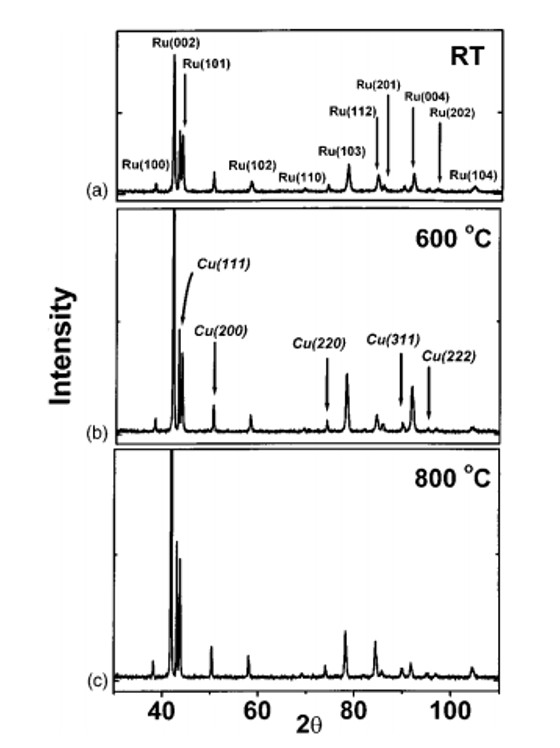
\includegraphics[width=0.5\textwidth]{3.jpg}
	\caption{Cu/Ru体系下的不同温度XRD图像}
	\label{Fig:3}
\end{figure}


但是显然更高温度的退火就会让Cu/Ru/$SiO_2$体系失效,一般认为这样的失效原因为
失效出现在高退火温度下,是由多晶硅化钌的形成引发的,进一步促进铜向硅衬底的扩散,形成铜硅化物突起。
从而导致阻挡层失效的。


在某种程度上,钌薄膜的质量对铜的相互扩散行为有决定性的影响。钌晶界的存在是
缺陷位点,大大加速了铜通过钌阻挡层的相互扩散。图\ref{Fig:4}(a)证明使用
Ru薄膜作为Cu扩散屏障层的失败是由于其柱状颗粒结构,促进了铜原子在高温下穿透硅衬
底。他们的横断面透射电子显微镜(TEM)结果清楚地显示了在硅衬底上垂直取向的Ru薄膜
的柱状微观结构。在550◦C退火后,Ru薄膜从Si衬底中分离,Cu通过Ru柱状晶界进入下面的
Si中,导致Cu/Ru/Si体系的降解。

\begin{figure}[htb]
	\centering
	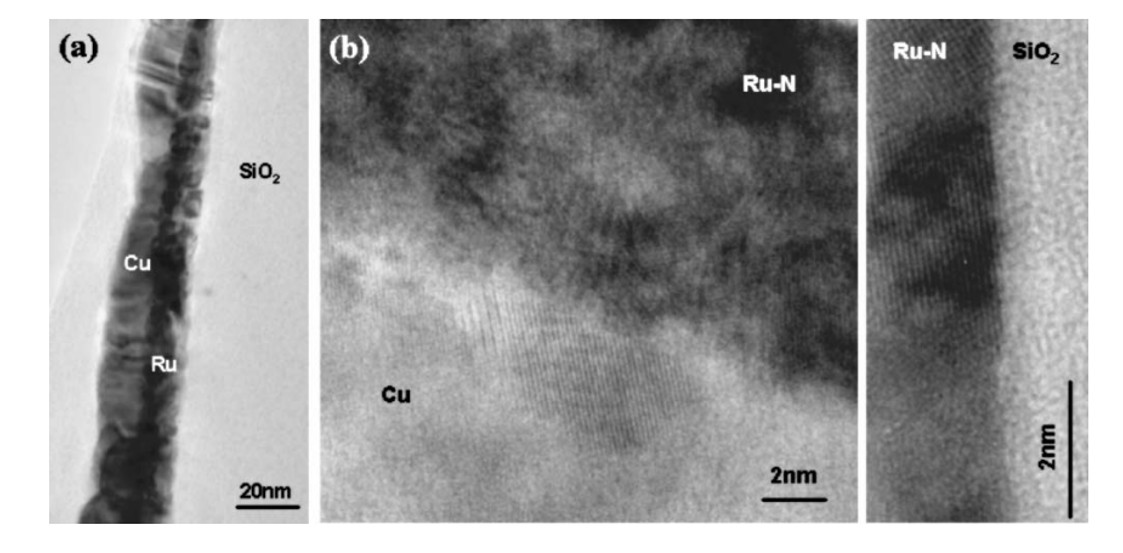
\includegraphics[width=0.8\textwidth]{4.jpg}
	\caption{TEM图像(a)Cu/Ru/$SiO_2$ (b)Cu/Ru-N/$SiO_2$}
	\label{Fig:4}
\end{figure}


可以观察到透射电子显微镜的结果清楚地显示了在硅衬底上垂直取向的Ru薄膜的柱状微观结构。
在550◦C退火后,Ru薄膜从Si衬底中分离,Cu通过Ru柱状晶界渗透到下面的Si中,导致Cu/Ru/Si
体系的降解。


然而,在Ru薄膜中引入异物会导致非晶态结构的形成,从而消除柱状结构的形成,控制晶界,最终
提高铜的相互扩散阻力。图\ref{Fig:4}(b)(c)证明,氮溶解到Ru薄膜中形成了具有10倍高薄片电阻
的非晶结构,掺杂延迟了钌硅化物的形成,减少了铜向介质层的扩散。进行N掺杂之后Cu/Ru表面的粘附性没有
明显的变化但是Ru/$SiO_2$明显没有柱状的颗粒所创造的间隙,而是彼此之间紧密贴合的粘连在了
一起。



\subsection{掺杂的Ru阻挡层}

在前一节提到了在Ru薄膜中引入杂质会导致非晶态结构的形成,从而消除柱状结构的形成,控制晶界,最终提高铜的
相互扩散阻力。并且给出了TEM图整明在Ru-N/$SiO_2$体系中相比与Ru/$SiO_2$粘附性有显著的
提升,不存在任何的柱状颗粒,认识具有清晰完整的晶向边界,不存在Cu向$SiO_2$的轻易扩散。


\begin{figure}[htb]
	\centering
	\begin{minipage}[t]{0.5\textwidth}
	\centering
	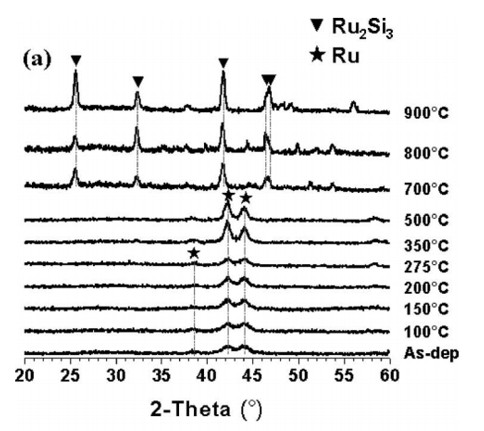
\includegraphics[width=0.8\textwidth]{5.jpg}
	\caption{XRD谱图 Ru/Si}
	\label{Fig:5}
	\end{minipage}
	\begin{minipage}[t]{0.45\textwidth}
	\centering
	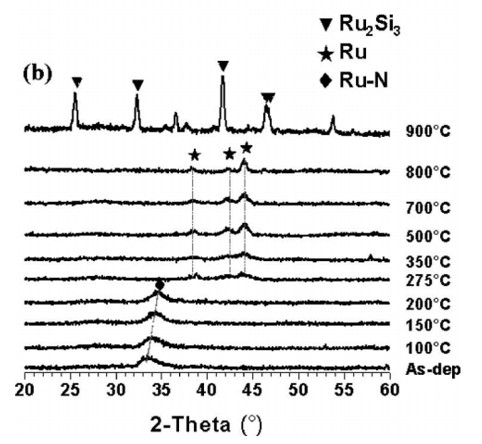
\includegraphics[width=0.8\textwidth]{6.jpg}
	\caption{XRD谱图 Ru-N/Si}
	\label{Fig:6}
	\end{minipage}
\end{figure}

如图\ref{Fig:5}所示,由于Ru/$SiO_2$体系的粘附力较差,所以在较低温度($500^oC$)情况下进行退火
就已经开始出现了$Ru_2Si_3$化合物,相对对于Cu/Ru体系$800^oC$都不会时出现新晶向的体系来说有明显的差距。
但是通过在Ru生长中掺杂N之后形成的Ru-N/$SiO_2$体系中Ru-N与$SiO_2$之间粘附紧密,有明显的晶界而不会出现
柱状的颗粒从而更容易保持稳定。所以可以在高达$800^oC$情况下进行退火保持晶向稳定,不出现Ru的硅化物。


掺杂杂质使得Ru与$SiO_2$的原理总的来说也很简单,就是通过一些外来元素例如硼(B)、磷(P)和碳
(C)能够诱导非晶态Ru薄膜的形成,从而显著提高了Ru薄膜防止Cu相互扩散的能力。在低κ介电层上
沉积了12 nm的Ru (P)薄膜,有效地阻止了铜在800◦C、5 min条件下扩散到硅片中。有些研究证明,
在热退火条件下,Ru-B-C的5 nm薄膜形成非晶相的温度明显高于纯Ru,掺杂膜在750◦C时热稳定。
金属元素也可以作为掺杂剂,与Ru形成非晶结构,提高其热稳定性。


但是这样的掺杂存在的主要问题就是通过掺杂确实可以让Ru与low-k介质的粘附变得稳定但是也极大的影响
了Ru的电阻率,Ru-N阻挡层的电阻率被极大的提升了甚至远超过正常的Ta/TaN体系。这使得Ru系金属
在作为阻挡层方面对比传统的阻挡层材料Ta/TaN 没有明显的优势,所以在经过一段时间的热潮之后
便逐渐落寞,很少有人继续研究下去了。但是Ru的低电阻率与对Cu高的粘附性的特点将会对接下来的
工艺研究起到重要的作用。


\section{基于AS-ALD工艺的Ru互连}


\begin{figure}[htb]
	\centering
	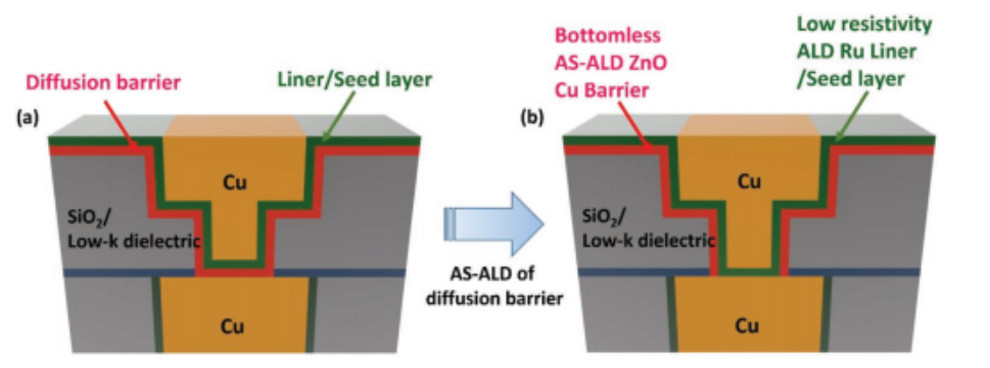
\includegraphics[width=1\textwidth]{7.jpg}
	\caption{(a)传统通孔结构示意图 (b)利用AS-ALD生长ZnO/Ru阻挡层结构示意图}
	\label{Fig:7}
\end{figure}


\subsection{DDT选择性验证}


\begin{figure}[htb]
	\centering
	\begin{minipage}[t]{0.5\textwidth}
	\centering
	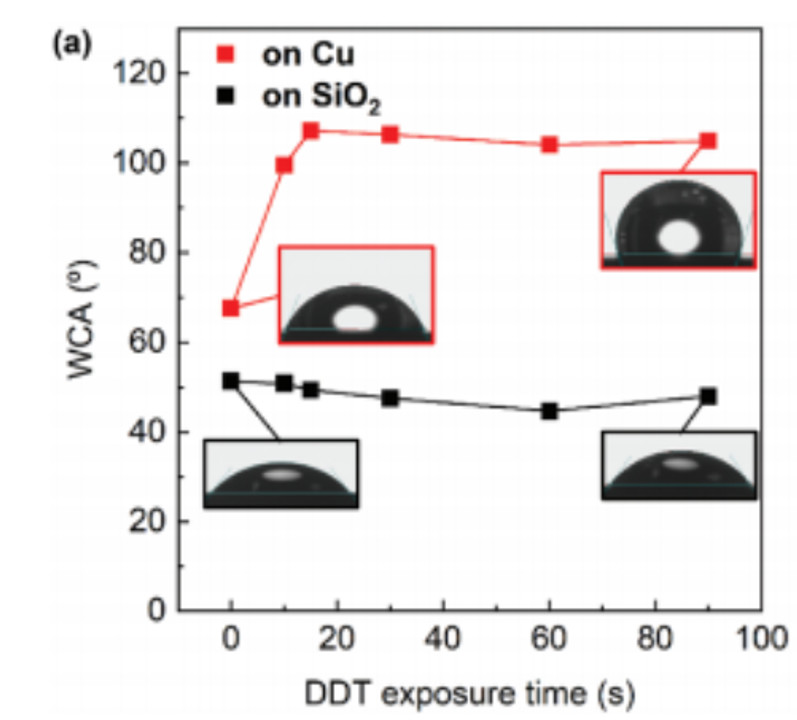
\includegraphics[width=0.8\textwidth]{8.jpg}
	\caption{在$120^oC$条件下将Cu与$SiO_2$浸泡DDT的浸润角区别}
	\label{Fig:8}
	\end{minipage}
	\begin{minipage}[t]{0.45\textwidth}
	\centering
	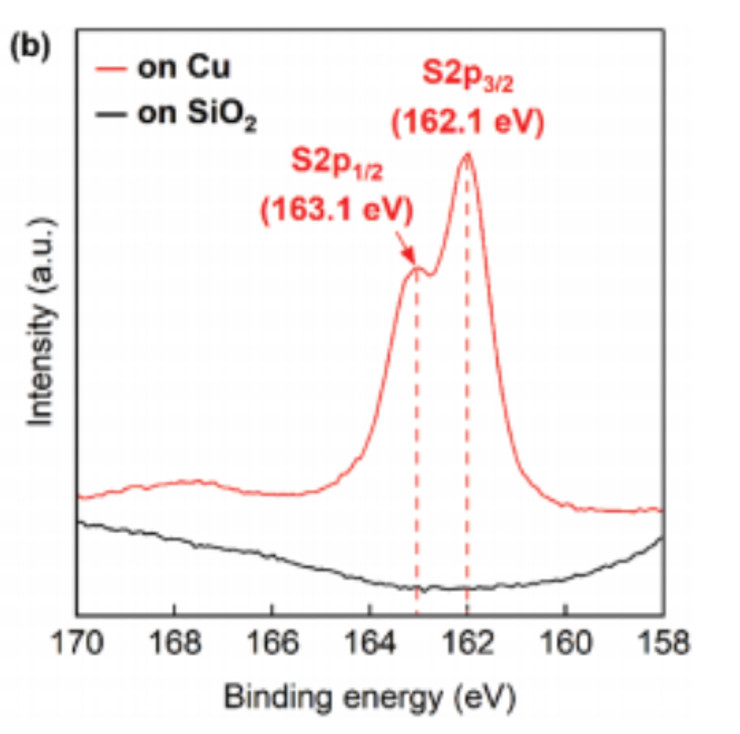
\includegraphics[width=0.8\textwidth]{9.jpg}
	\caption{经过DDT浸泡后Cu与$SiO_2$的XPS光谱峰值}
	\label{Fig:9}
	\end{minipage}
\end{figure}



\subsubsection{DDT选择性吸附}


\begin{figure}[htb]
	\centering
	\begin{minipage}[t]{0.3\textwidth}
	\centering
	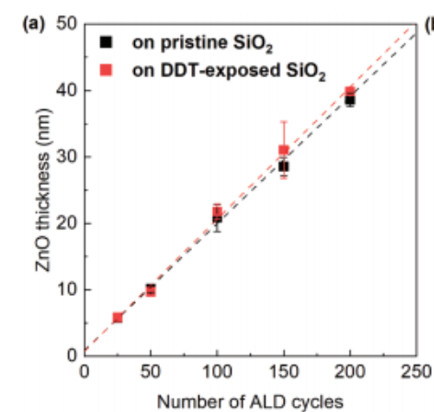
\includegraphics[width=0.8\textwidth]{10.jpg}
	\label{Fig:10}
	\end{minipage}
	\begin{minipage}[t]{0.3\textwidth}
	\centering
	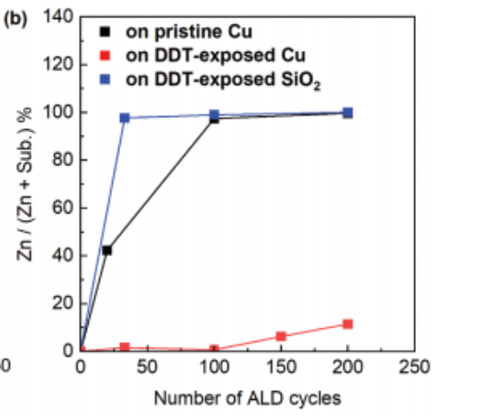
\includegraphics[width=0.9\textwidth]{11.jpg}
	\label{Fig:11}
	\end{minipage}
	\begin{minipage}[t]{0.3\textwidth}
	\centering
	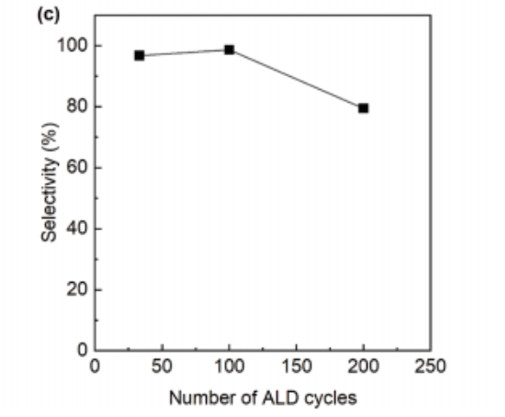
\includegraphics[width=1\textwidth]{12.jpg}
	\label{Fig:12}
	\end{minipage}
	\caption{(a)$SiO_2$分别浸泡DDT与不浸泡情况下ZnO生长情况 (b)
	Cu分别浸泡DDT与不浸泡情况下ZnO生长后的元素比与浸泡过DDT的$SiO_2$对比 (c)浸泡过DDT的Cu和$SiO_2$结构生长ZnO的ALD循环次数
	与最终生长选择比}
\end{figure}



\subsubsection{DDT去除}


\begin{figure}[htb]
	\centering
	\begin{minipage}[t]{0.5\textwidth}
	\centering
	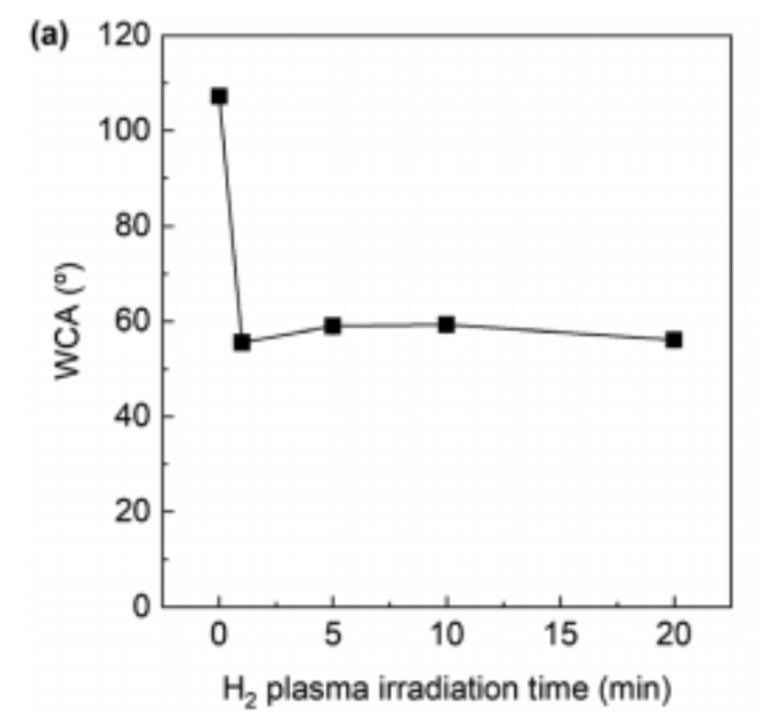
\includegraphics[width=0.8\textwidth]{13.jpg}
	\caption{经过$H_2$条件下$150^oC \quad 5 min$处理后的Cu表面的浸润角测量}
	\label{Fig:13}
	\end{minipage}
	\begin{minipage}[t]{0.45\textwidth}
	\centering
	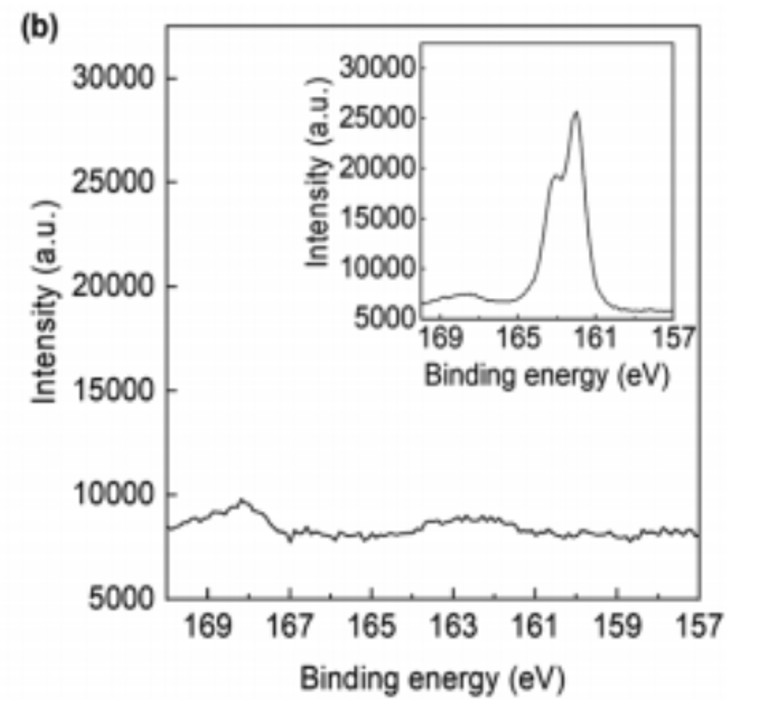
\includegraphics[width=0.8\textwidth]{14.jpg}
	\caption{经过$H_2$条件下$150^oC \quad 5 min$处理后的表面XPS光谱,右上角小窗为Cu表面,其他部分为$SiO_2$表面}
	\label{Fig:14}
	\end{minipage}
\end{figure}





\subsection{AS-ALD选择性生长}


\begin{figure}[htb]
	\centering
	\begin{minipage}[t]{0.45\textwidth}
	\centering
	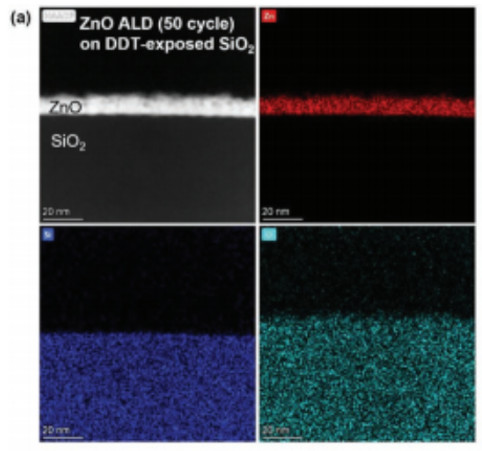
\includegraphics[width=0.8\textwidth]{15.jpg}
	\label{Fig:15}
	\end{minipage}
	\begin{minipage}[t]{0.45\textwidth}
	\centering
	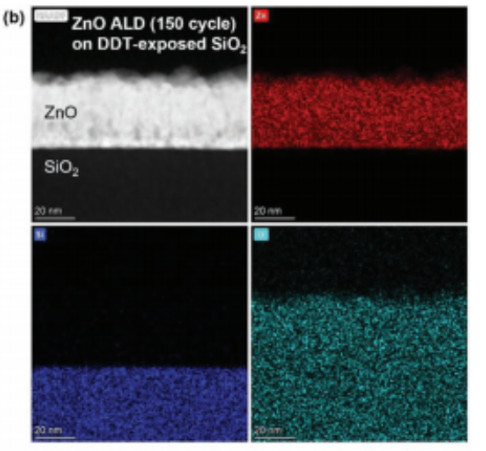
\includegraphics[width=0.9\textwidth]{16.jpg}
	\label{Fig:16}
	\end{minipage}
	\begin{minipage}[t]{0.45\textwidth}
	\centering
	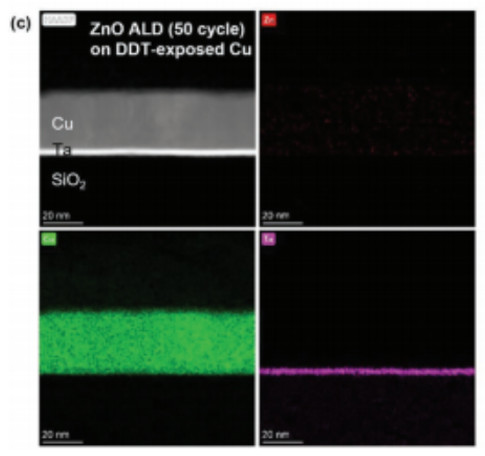
\includegraphics[width=1\textwidth]{17.jpg}
	\label{Fig:17}
	\end{minipage}
	\begin{minipage}[t]{0.45\textwidth}
	\centering
	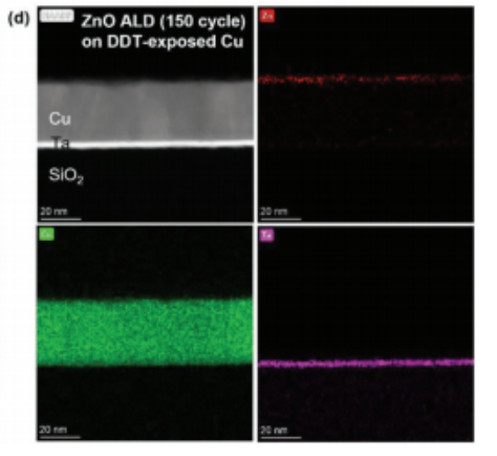
\includegraphics[width=1\textwidth]{18.jpg}
	\label{Fig:18}
	\end{minipage}
	\caption{TEM图像与EDS图像mapping (a)在DDT浸泡后的$SiO_2$生长ZnO-ALD(50 cycles) 
	(b)在DDT浸泡后的$SiO_2$生长ZnO-ALD(150 cycles) (c)在DDT浸泡后的Cu生长ZnO-ALD(50 cycles)
	 (d)在DDT浸泡后的Cu生长ZnO-ALD(50 cycles)}
\end{figure}



\begin{figure}[htb]
	\centering
	\begin{minipage}[t]{0.5\textwidth}
	\centering
	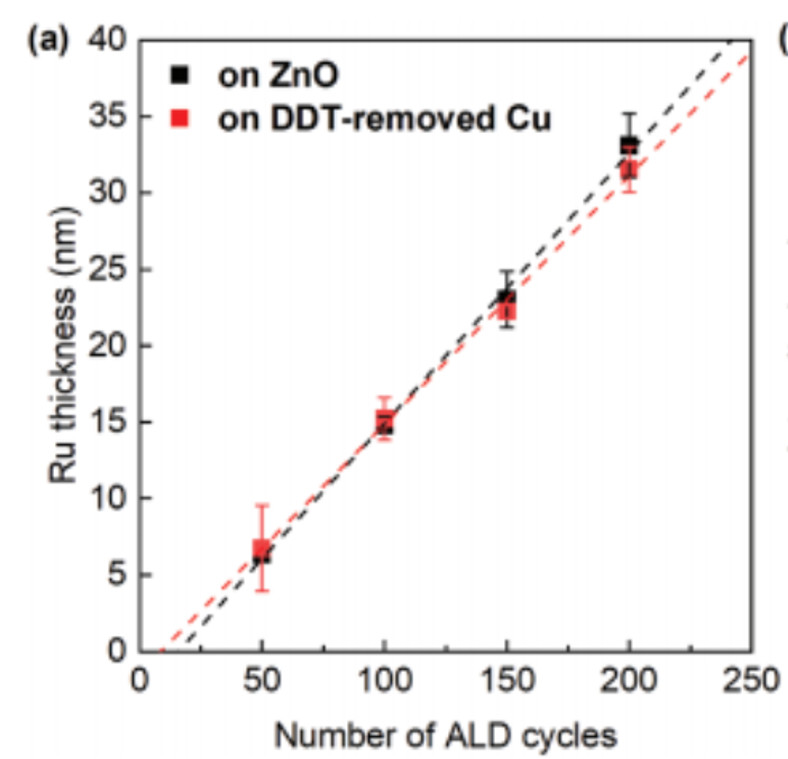
\includegraphics[width=0.8\textwidth]{19.jpg}
	\caption{在ZnO表面与在经过DDT浸泡并移除后的Cu表面ALD生长Ru的厚度与循环关系}
	\label{Fig:19}
	\end{minipage}
	\begin{minipage}[t]{0.45\textwidth}
	\centering
	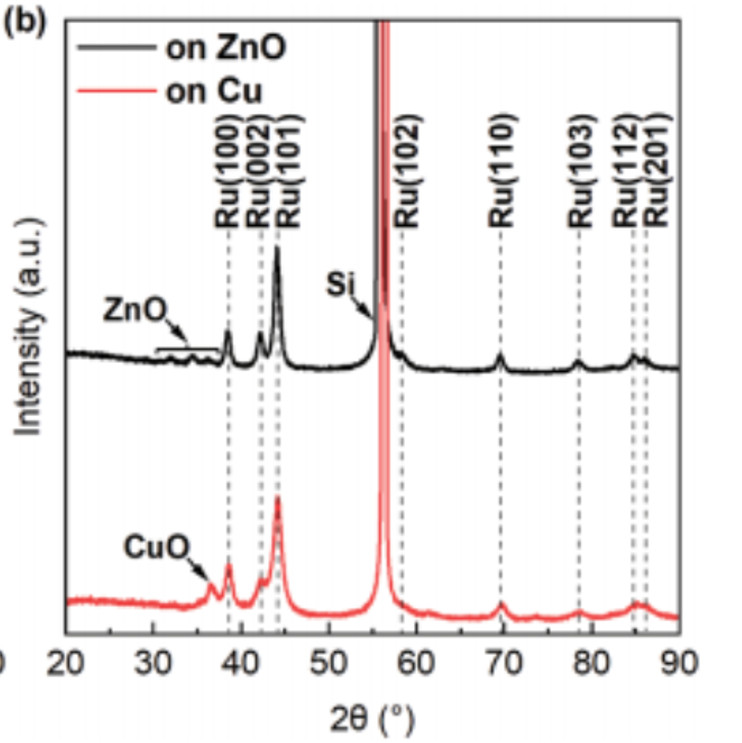
\includegraphics[width=0.8\textwidth]{20.jpg}
	\caption{在ZnO表面与在经过DDT浸泡并移除后的Cu表面ALD生长Ru的XRD图谱}
	\label{Fig:20}
	\end{minipage}
\end{figure}


\subsection{工艺性能表征}


\begin{figure}[htb]
	\centering
	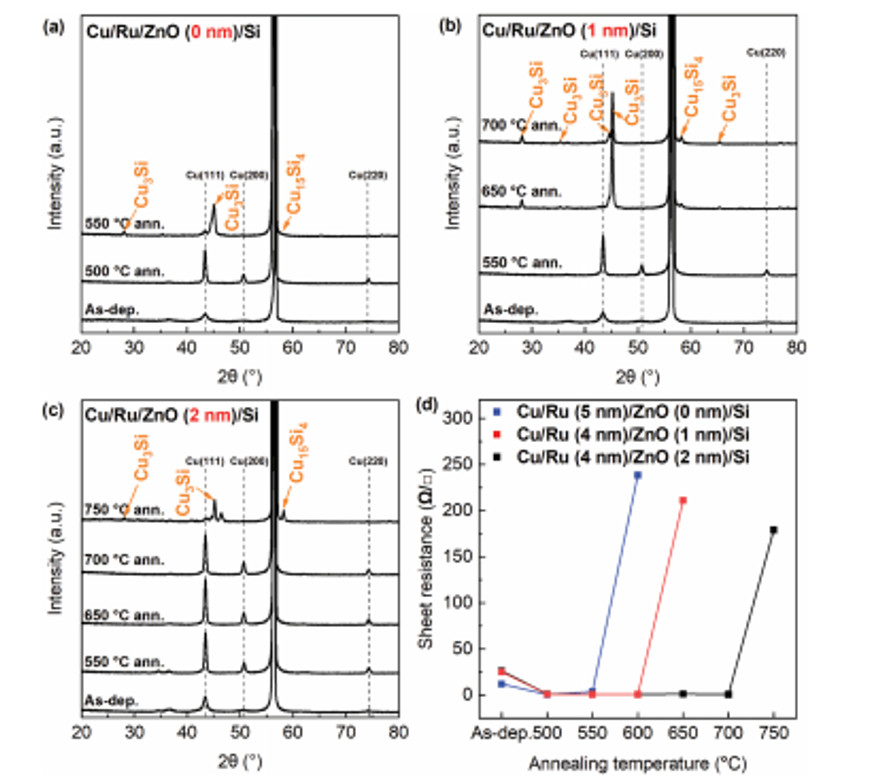
\includegraphics[width=0.8\textwidth]{26.jpg}
	\caption{(a)Cu(60nm)/Ru(4nm)/ZnO(0nm)不同温度下退火XRD图谱 (b)Cu(60nm)/Ru(4nm)/ZnO(1nm)不同温度下退火XRD图谱 
	(c)Cu(60nm)/Ru(4nm)/ZnO(2nm)不同温度下退火XRD图谱 (d)不同温度退火情况下不同ZnO厚度的方阻变化}
	\label{Fig:26}
\end{figure}




\section{Ru阻挡层工艺与其他工艺对比}


\begin{figure}[htb]
	\centering
	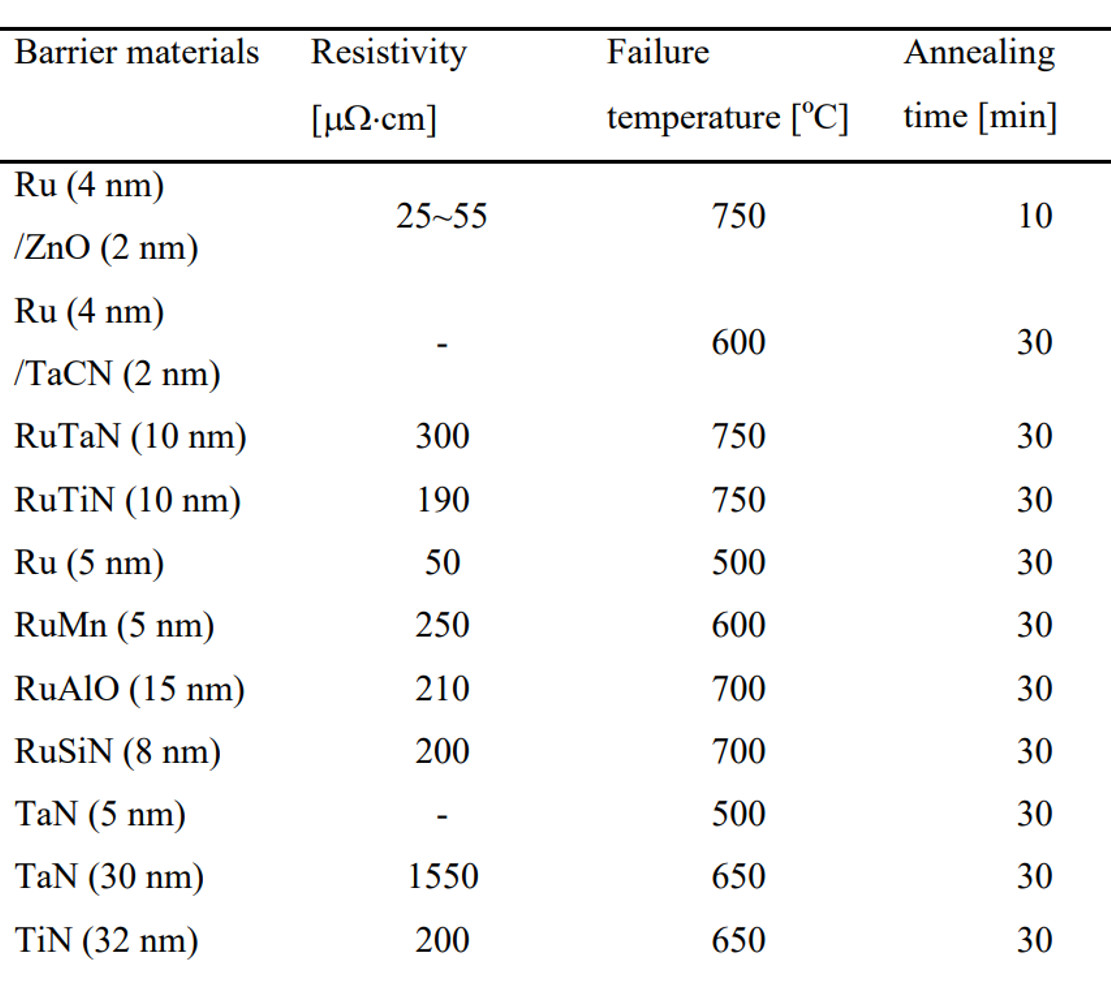
\includegraphics[width=0.8\textwidth]{25.jpg}
	\caption{不同阻挡层之间性质对比}
	\label{Fig:25}
\end{figure}


% \begin{lstlisting}[title=Myfile, frame=shadowbox]
%  numbers=left, 
%     numberstyle= \tiny, 
%     keywordstyle= \color{ blue!70},
%     commentstyle= \color{red!50!green!50!blue!50}, 
%     frame=shadowbox, % 阴影效果
%     rulesepcolor= \color{ red!20!green!20!blue!20} ,
%     escapeinside=``, % 英文分号中可写入中文
%     xleftmargin=2em,xrightmargin=2em, aboveskip=1em,
%     framexleftmargin=2em
% % 代码段
% \end{lstlisting}

% \begin{figure}[htb]
% 	\centering
% 	\includegraphics[width=0.5\textwidth]{xiaohui.eps}
% 		\caption{我国鼠疫自然疫源地的地理分布}
% \label{fig:xiaohui}
% \end{figure}
  
% Paste your own text here and click the 'Check Text' button. Click the colored 
% phrases for details on pot ential errors. or use this text too see an few of of the 
% problems that LanguageTool can detect. What do you thinks of grammar 
% checkers? Please not that they are not perfect. \cite{approach,hart1968formal}Style issues get a blue marker: It's 
% 5 P.M. in the afternoon. LanguageTool 3.8 was released on Thursday, 27 June 
% 2017.\cite{hart1968formal}
% \begin{center}
% 	\begin{longtable}{|c|c|c|c|}
% 		\caption{A simple longtable example}\\
% 		\hline
% 		\textbf{First entry} & \textbf{Second entry} & \textbf{Third entry} & \textbf{Fourth entry} \\
% 		\hline
% 		\endfirsthead
% 		\multicolumn{4}{c}%
% 		{\tablename\ \thetable\ -- \textit{Continued from previous page}} \\
% 		\hline
% 		\textbf{First entry} & \textbf{Second entry} & \textbf{Third entry} & \textbf{Fourth entry} \\
% 		\hline
% 		\endhead
% 		\hline \multicolumn{4}{r}{\textit{Continued on next page}} \\
% 		\endfoot
% 		\hline
% 		\endlastfoot
% 		1 & 2 & 3 & 4 \\ 1 & 2 & 3 & 4 \\ 1 & 2 & 3 & 4 \\ 1 & 2 & 3 & 4 \\
% 		1 & 2 & 3 & 4 \\ 1 & 2 & 3 & 4 \\ 1 & 2 & 3 & 4 \\ 1 & 2 & 3 & 4 \\
% 	\end{longtable}
% \end{center}

% \begin{center}
% 	\begin{longtable}{|p{1cm}|p{2cm}|p{3cm}|p{4cm}|}
% 		\hline
% 		\#&指令&描述&使用场景\\ \hline \hline
% 		\endhead
% 	\end{longtable}
% \end{center}

% \begin{center}
% 	\begin{tabular}{|p{5cm}|p{6cm}|}
% 		\hline
% 		\multicolumn{2}{|p{11cm}|}{\textbf{Class  CalendarItem:}该类继承自Calend}\\ \hline
% 		set(String)& 参数为用户新加入的事项,用于修改text。\textcolor{red}{注意传入的为null,抛出自定义异常}\\ \hline
% 	\end{tabular}
% \end{center}

\newpage
\addcontentsline{toc}{section}{参考文献}
\bibliography{course-template}%记得需要F8
\end{document}